\chapter{ Аналитический раздел}
\label{cha:analysis}

\textit{SDR(Standart Dynamic Range) изображение} -- изображение, пиксели которого содержат цвета и яркость, соответствующую глубине монитора.

\textit{LDR(Low Dynamic Range) изображение} -- изображение, пиксели которого хранят ограниченный диапазон цветов и яркости, предназначенное для отображении на старых мониторах.

\textit{HDR(High Dynamic Range) изображение} -- изображение, пиксели которого содержат более широкие значения цвета и яркости в сравнении с изображениями стандартного диапазона(SDR).

\textit{Глубина цвета} -- количество бит, приходящихся на один пиксель 

\section{ Различия LDR и HDR изображений}
    
    Несмотря на то, что технологии за послдение несколько лет быстро развиваются и качество полученных кадров и устройств, их отображающих, увеличивается, получение картинки, сопоставимой с реальным окружением, остается нелегкой задачей. Яркость, диапазон цветов, которые видит человек в повседневной жизни, невозможно отобразить на большинстве мониторов, используещихся во всем мире. 

    Хотя уже начинают появлятся так называемые HDR мониторы и существуют камеры, сенсоры которых позволяют запечатлить широкий спектр цветов, яркостей и деталей, цена таких устройств может достигать огромных значений, поэтому большинство мониторов остаются SDR формата и не в состоянии передать картинку с большим количеством цветовой информации.

    Глубина цвета на большинстве мониторов составляет 8 бит. Глубина цвета самого распространенного формата изображений JPEG так же составляет 8 бит, в котором используется цветовое пространстов $YC_rC_b$. Это цветовое пространство позволяет использовать лишь малую часть видимых человеком цветов. Так же это цветовое пространство не способно передать большую часть яркостей, которых способен распознать человеческий глаз.

    В противовес формату JPEG существует так называемый RAW формат. В отличии от JPEG он способен содержать гораздо больше информации. Глубина цвета такого формата может достигать 12-16 бит(Значение может варьироваться в зависимости от возможностей сенсора камеры), который доступен в большинстве современных камер. Чаще всего этот формат автоматически переводят в JPEG во время съемки, что приводит к потере многих деталей без возможности восстановления. Однако, используя специальные инструменты RAW изображение в дальнейшем можно преобразовать в LDR изображение, получив на выходе кадр без потери нужной информации(провести tonemapping).

    На цветовом пространстве \ref{fig:hdrdiff} наглядно показан охват возможных отображаемых цветов в RGB пространстве или на тех же LDR мониторах и в HDR с глубиной цвета хотя бы в 12 бит.

\begin{figure}[ht!]
    \centering{
        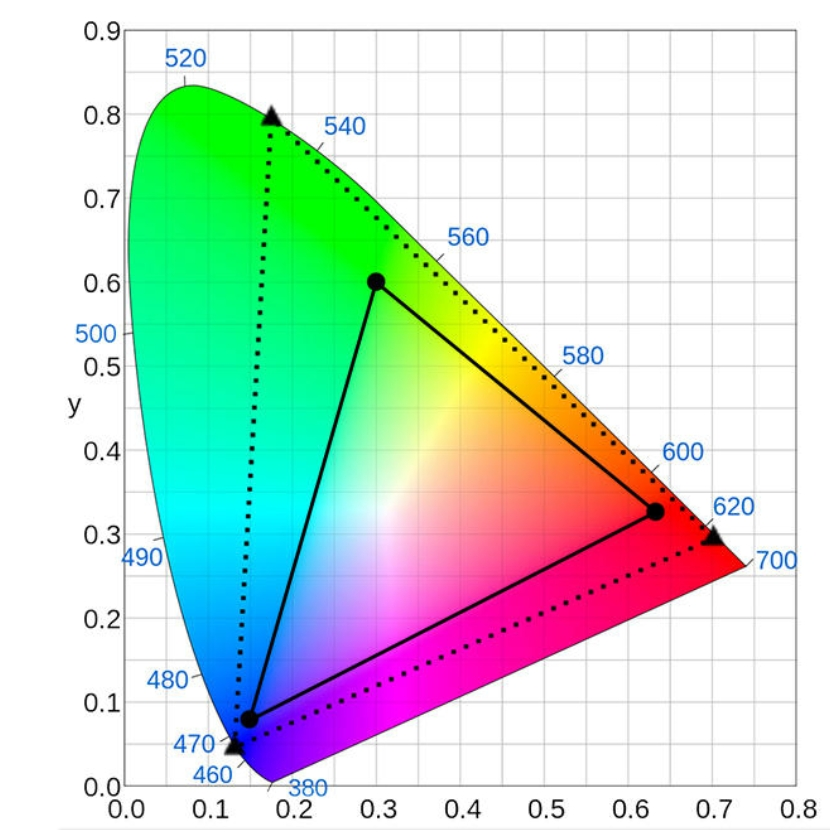
\includegraphics[width=0.4\textwidth]{img/rgb_vs_hdr_gamut.jpg}
	\caption{Охват видимых человеком цветов цветовым пространством RGB и HDR.}
        \label{fig:hdrdiff}
        }
\end{figure}

    Главное различие HDR и традиционных LDR изображений в том, что HDR картинка не зависит от какого-либо устройства и содержит максимально большое количество информации. Количество отображаемой информации на устройстве уже зависит непосредственно от его собственных характеристик и возможностей. LDR изображение же зависит от устройства, на котором оно будет отображаться и спроектировано специально под мониторы или экраны, которые отображают определенное количество цветовой информации.

\section{ Процесс получения HDR изображения}

HDR изображение можно получить несколькими способами: 
\begin{itemize}
    \item c помощью объединения снимков с разной длинной экспозиции,
    \item с помощью камеры, сенсор который позволяет захватить широкий объем данных,
    \item при помощи перевода LDR изображения в HDR специальными алгоритмами
\end{itemize}

Первый метод является более распространенным, так как устройства, которые больше всего распространены в повседневной жизни(телефоны, планшеты, веб-камеры) не обладают достаточно мощными сенсорами, для того, чтобы захватить широкий диапазон цветов. Последний метод не получил распространения, потому что задача перевода LDR или SDR изображения в HDR возможна только при помощи преминения алгоритмов реконструкции, завязанных на нейронных сетях, появившихся достаточно недавно.

\subsection { Конвейер получения HDR изображения на камере со слабым сенсором}
\begin{itemize}
    \item Выравнивание кадров,
    \item Реконструкция и удаление движущихся объектов(артефактов),
    \item Слияние кадров с разной экспозицией,
    \item Преобразование HDR к LDR(tonemapping) если это требуется
\end{itemize}

Наглядно процесс получения HDR кадра с возможностью перевода его в LDR показан на схеме \ref{fig:hdrpipeline}

\begin{figure}[ht!]
    \centering{
        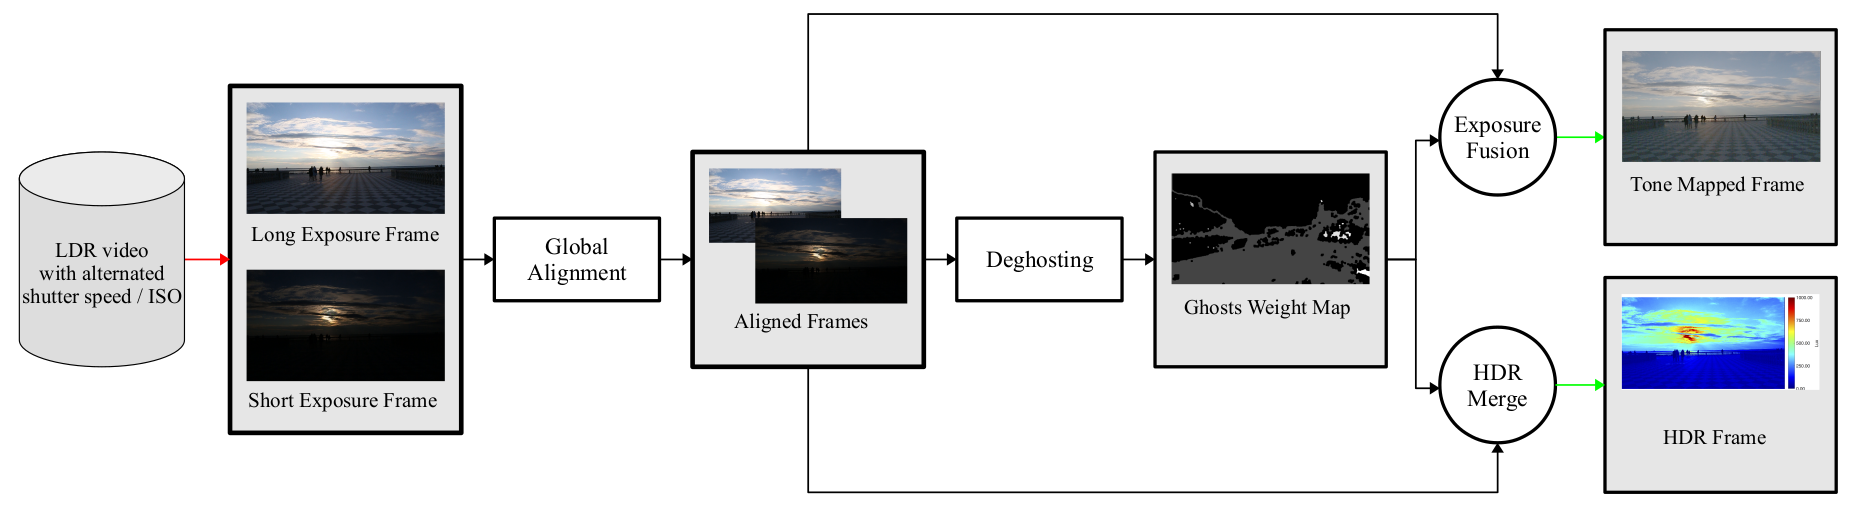
\includegraphics[width=1\textwidth]{img/hdrpipeline.png}
	\caption{Процесс получения HDR изображения путем слияния кадров с разной экспозицией}
        \label{fig:hdrpipeline}
        }
\end{figure}

\subsection{ Получение HDR видео на камере со слабым сенсором в режиме реального времени}
    
    Данная задача подразумевает собой быстрое создание HDR изображений из 2-3 кадров с изменяещейся экспозицией, которые получаются, путем изменения экспозиции через каждый последующий кадр. Таким образом, можно быстро получить два кадра, которые будут содержать всю информацию о самых темных и самых светлых участках сцены. Так, как эти кадры следуют друг за другом, различия в них, предполагается, будут незначительными.

    При записи видео в таком формате очень важна скорость алгоритмов, использующихся при получении HDR кадра. Операции выравнивания, удаления артефактов, слияния кадров и преобразование полученного кадра в LDR должны протекать быстро.

\subsubsection{ Способы получения разной экспозиции в видео}
    Получение разной экспозиции кадров можно добиться несколькими способами:
\begin{enumerate}
    \item Использовать несколько камер, каждая из которых будет вести запись с соответствующей экспозицией;
    \item Использовать камеру с нескольким сенсорами, каждыдй из которых будет вести запись с соответствующей экспозицией;
    \item Использовать одну камера, меняя параметр выдержки или ISO, которые влияют на полученную экспозицию;
\end{enumerate}

    Первые два способа позволяют сохранить количество кадров в секунду и улучшить качество получаемой картинки, но они требуют предварительной калибровки. Так же несколько камер и камеры с дополнительными сенсорами не самые распространенные решения в телефонах и других гаджетах.
    
    Третий способ позволяет получать кадры с разной экспозицией на любом устройстве, в котором есть камера, что делает его более универсальным, но это снижает количество кадров в секунду почти в два раза.

\section{ Выравнивание изображений}
    Первым шагом в получении HDR изображения является глобальное выравнивание последовательности кадров с разной экспозицией. Предполагается, что 2 соседних кадра не меняются слишком быстро.

    Но при съемке с рук или при съемке в движении, кадры все равно меняются, положение записывающего устройства тоже может быть нестабильным. В дальнейших шагах получения HDR снимка очень важно, чтобы кадры с разной экспозицией были максимально выровнены по отношению друг к другу. 

    Задача выравнивания усложняется тем, что экспозиции изображений сильно разнятся. Для решения этой задачи используется алгоритм MTB(Median Threshold Bitmap) пороговое отсечение по медианному значению.

\subsection{ Алгоритм MTB(Median Threshold Bitmap)}
    На вход алгоритму подается N 8-битных монохромных изображений, которые можно получить путем использования зеленого канала изображения, либо путем перевода каждого пикселя 24-битного sRGB изображения в серый цвет с помощью выражения \ref{eq:grayscale}
\begin{equation}
    \centering{
        grey = \frac{(54*red + 183*green + 19*blue)}{256}}
    \label{eq:grayscale}
\end{equation}

    Одно из изображений выбирается базовым. Остальные N-1 при выравнивании будут опираться на базовое.

    Далее требуется для каждого из изображений:
\begin{enumerate}
    \item Найти среднее значение(8-битное значение) из гистограммы низкого разрешения пикселей монохромного изображения. 
    \item Создать растровое изображения, в котором 0 будут отмечаться пиксели, которые меньше или равны среднему значению и 1 будут отмечаться пиксели, которые строго больше этого среднего значения.
\end{enumerate}

    Результаты этоих шагов представленны на примере двух изображений с разной экспозицией \ref{fig:bitmapExample}

\begin{figure}[ht!]
    \centering{
        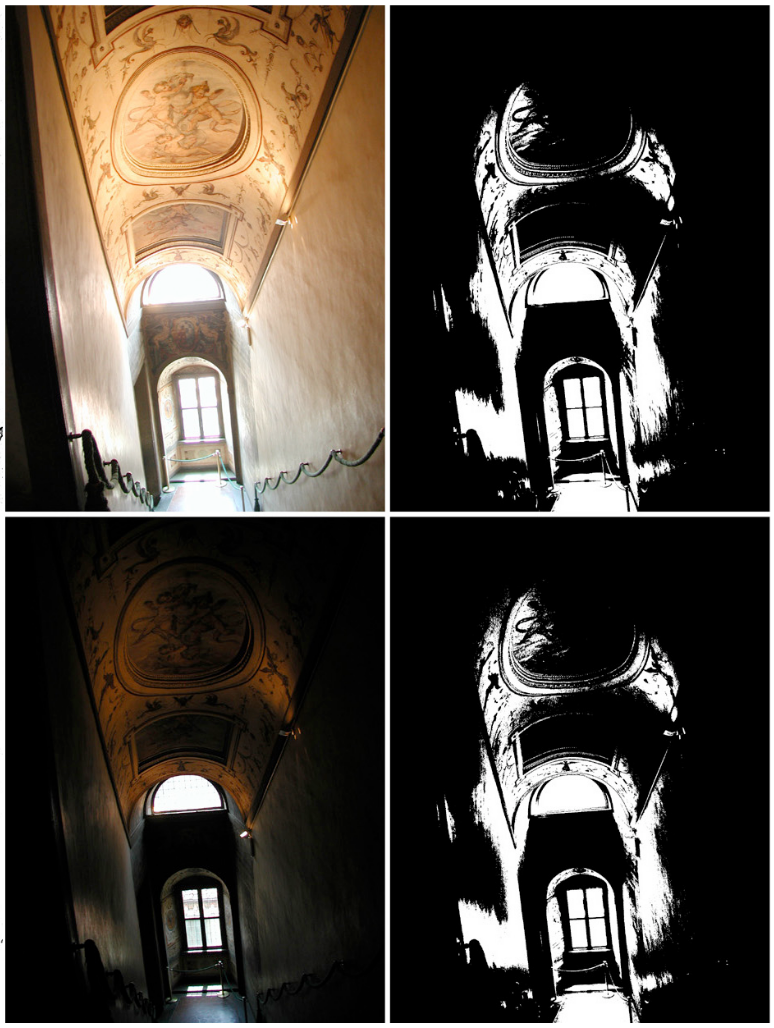
\includegraphics[width=1\textwidth]{img/bitmapExample.png}
	\caption{ Получение растровых изображений, использующихся для дальнейшего сравнения(справа), оригиналы изображений(слева)}
        \label{fig:bitmapExample}
        }
\end{figure}

    После этого каждое N-1 изображение подгоняется под базовое. Вначале они сравниваются. Сравнение происходит путем побитовой операции XOR -- каждый пиксель изображения высчитывается с каждым соответствующем пикселем базового изображения операцией XOR. Результаты сохраняются и на выходе получается очередное растровое изображение, в котором 0 - пиксели, информация которых совпала с базовым изображением и 1 - пиксели, информация которых не совпала.

    Для выравнивания находится значение сдвига (x, y): x - смещение изображения по горизонтали, y - сдвиг изображения по вертикали.
Самый оптимальный сдвиг будет тот, у которого при сравнение изображения с базовым, количество пикселей 1 будет минимальное. Искать его можно несколькими способами. Самый очевидный - простой перебор всевозможных сдвигов (x, y), но используется более оптимальный метод. С помощью пиромидальной сегментации изображения можно добиться наименьшего количества сравнений двух растровых побитово размеченных изображений.

Каждое монохромное изображение переводится на следующий уровень путем уменьшения его разрешения в два раза. Таким образом получаем несколько уровней, которые содержат монохромные изображения. Начиная с самого последнего уровня(изображения которых содержат наименьшее разрешение) нужно найти для них растровое изображение по медианному значению и найти сдвиг перебором по значениям +-1 пиксель в каждом направлении(по горизонтали и вертикали)

На следующем уровне "пирамиды" нужно домножить полученный сдвиг на 2(значение, на которое менялось разрешение на каждом уровне пирамиды) и снова вычислить наилучший сдвиг на расстоянии +-1 пиксель от текущего сдвига в разные направления x и y.

Эти действия продолжаются до последнего(изначального) уровня пирамиды, на котором получается окончательный требуемый сдвиг (x, y) для изображения, чтобы быть выравненным по отношению к базовому.
